\documentclass[conference]{IEEEtran}
\IEEEoverridecommandlockouts

% === Core IEEE packages ===
\usepackage{cite}
\usepackage{amsmath,amssymb,amsfonts}
\usepackage{algorithmic}
\usepackage{graphicx}
\usepackage{textcomp}
\usepackage{xcolor}

% === Additional packages ===
\usepackage{booktabs}
\usepackage{multirow}
\usepackage{array}
\usepackage{tabularx}
\usepackage{algorithm}
\usepackage{listings}
\usepackage{balance}
\usepackage{url}
\usepackage{tikz}
\usetikzlibrary{shapes.geometric, arrows.meta, positioning, fit, calc}
\usepackage[bookmarks=false]{hyperref}

% === Listings style ===
\lstset{
  basicstyle=\footnotesize\ttfamily,
  breaklines=true,
  frame=single,
  captionpos=b,
  numbers=left,
  numberstyle=\tiny,
  numbersep=5pt,
  xleftmargin=10pt,
  tabsize=2
}

\def\BibTeX{{\rm B\kern-.05em{\sc i\kern-.025em b}\kern-.08em
    T\kern-.1667em\lower.7ex\hbox{E}\kern-.125emX}}

\begin{document}

\title{Tree-Grounded Generation: Agentic Document Tree Exploration as an Alternative to Embedding-Based Retrieval-Augmented Generation}

\author{
  \IEEEauthorblockN{Suhaib Ahmad}
  \IEEEauthorblockA{
    \textit{Independent Researcher} \\
    suhaib@example.com}
}

\maketitle

% =====================================================================
% ABSTRACT
% =====================================================================
\begin{abstract}
Retrieval-Augmented Generation (RAG) has become the dominant paradigm for grounding large language model (LLM) outputs in external knowledge. However, traditional RAG pipelines depend on embedding-based similarity search over flat document chunks, which fundamentally discards hierarchical document structure, introduces chunk boundary artifacts, and suffers from embedding fragility across domains. We present \textbf{Tree-Grounded Generation (TGG)}, a retrieval paradigm that eliminates embedding-based similarity search entirely. TGG parses heterogeneous documents---PDFs, Markdown, Word, spreadsheets, and source code---into a \textit{Universal Document Tree} (UDT), a uniform hierarchical representation that preserves the original structural semantics of each document type. An LLM agent then navigates these trees using seven specialized exploration tools, making deliberate retrieval decisions guided by query-adaptive budget estimation. We describe the architecture, formalize the agent exploration protocol, and present a systematic comparative analysis against traditional RAG, agentic RAG, and graph-based retrieval across twelve analytical dimensions. Our analysis demonstrates that TGG preserves structural context that embedding-based approaches systematically destroy, enables multi-hop reasoning through explicit tree traversal, and eliminates the operational overhead of vector database maintenance. We discuss the trade-offs of this approach, including increased LLM invocation costs and latency sensitivity, and identify conditions under which tree-grounded exploration is preferable to similarity-based retrieval.
\end{abstract}

\begin{IEEEkeywords}
retrieval-augmented generation, document tree, agentic retrieval, large language models, structured document parsing, tool-augmented reasoning
\end{IEEEkeywords}

% =====================================================================
% I. INTRODUCTION
% =====================================================================
\section{Introduction}

Large language models (LLMs) have demonstrated remarkable capabilities across language understanding and generation tasks~\cite{brown2020gpt3, vaswani2017attention}. However, their parametric knowledge is static, bounded by training data cutoffs, and prone to hallucination when confronted with queries requiring precise factual grounding. Retrieval-Augmented Generation (RAG)~\cite{lewis2020rag} addresses this limitation by coupling LLMs with external retrieval systems: documents are split into chunks, embedded into vector space, and retrieved via cosine similarity at query time.

While RAG has achieved widespread adoption, a growing body of evidence exposes fundamental limitations in its embedding-and-chunk architecture. Recent benchmarks show that even state-of-the-art RAG systems answer only 44\% of factual questions correctly when using straightforward retrieval~\cite{yang2024crag}, with legal research tools hallucinating 17--33\% of citations despite RAG augmentation~\cite{dho2025legalrag}. These failures are not incidental---they stem from structural properties of the RAG pipeline itself.

The core issue is \textit{structural erasure}. When a 200-page technical manual is split into 512-token chunks and projected into embedding space, the hierarchical relationships between sections, subsections, tables, figures, and cross-references are irreversibly destroyed. The retriever operates on a flat collection of text fragments with no awareness that Chapter~3 contains Section~3.2 which references Table~4.1 in the appendix. This structural information is precisely what humans rely on when navigating complex documents, and its loss degrades retrieval quality in predictable ways~\cite{multidocfusion2025, reconstructchunking2025}.

We propose \textbf{Tree-Grounded Generation (TGG)}, a retrieval paradigm that replaces embedding-based similarity search with \textit{agentic exploration of structured document trees}. Rather than pre-computing embeddings and retrieving chunks by proximity, TGG parses each document into a Universal Document Tree (UDT) that preserves its native hierarchical structure, then equips an LLM agent with navigation tools to explore these trees deliberately.

The key insight is that document retrieval is fundamentally a \textit{navigation} problem, not a \textit{similarity} problem. When a domain expert searches a technical specification for a particular parameter, they do not compute semantic similarity across all paragraphs---they consult the table of contents, navigate to the relevant section, scan for the parameter name, and follow cross-references as needed. TGG operationalizes this expert navigation behavior as an LLM agent protocol.

The contributions of this paper are as follows:
\begin{itemize}
    \item We propose TGG, a retrieval paradigm that grounds LLM answers in explicit document tree traversal rather than embedding similarity, eliminating the vector database dependency entirely.
    \item We design the Universal Document Tree (UDT), a uniform hierarchical schema that accommodates PDFs, Markdown, Word documents, spreadsheets, and source code within a single node-based representation.
    \item We formalize an agent exploration protocol with seven navigation tools and a query-adaptive budget estimation mechanism that adjusts exploration depth based on query complexity.
    \item We present a systematic comparative analysis of TGG against traditional RAG, agentic RAG variants, and graph-based retrieval across twelve analytical dimensions, identifying the conditions under which each approach is preferable.
\end{itemize}

The remainder of this paper is organized as follows. Section~II presents background on RAG and its known limitations. Section~III surveys related work in hierarchical retrieval, agentic retrieval, and graph-based approaches. Section~IV describes the TGG system architecture in detail. Section~V covers key implementation aspects. Section~VI presents our comparative analysis. Section~VII discusses limitations, and Section~VIII concludes.

% =====================================================================
% II. BACKGROUND AND MOTIVATION
% =====================================================================
\section{Background and Motivation}

\subsection{The RAG Pipeline}

The canonical RAG pipeline~\cite{lewis2020rag} operates in two phases. During \textit{indexing}, source documents are split into fixed-size chunks (typically 256--1024 tokens), each chunk is passed through an embedding model to produce a dense vector representation, and these vectors are stored in a vector database with associated metadata. During \textit{retrieval}, the user query is embedded using the same model, the top-$k$ most similar chunks are retrieved via approximate nearest neighbor search, and these chunks are prepended to the LLM prompt as context for answer generation.

Subsequent work has refined this pipeline into what surveys classify as Naive RAG, Advanced RAG (with pre-retrieval query rewriting and post-retrieval reranking), and Modular RAG (with pluggable retrieval, augmentation, and generation modules)~\cite{gao2024ragsurvey, ranjan2024ragsurvey}.

\subsection{Fundamental Limitations}

Despite these refinements, three structural limitations persist across all embedding-based RAG variants.

\textbf{Chunk Boundary Problem.} Fixed-size chunking splits documents at arbitrary token boundaries, fragmenting coherent arguments, splitting table rows from their headers, and separating conditional clauses from their antecedents. A clinical decision support study found that structure-aligned adaptive chunking achieved 87\% accuracy versus 13\% for fixed-size baselines on the same corpus~\cite{chunking2025clinical}, demonstrating that chunk boundaries are not merely an implementation detail but a primary source of retrieval error. Overlap-based mitigations (10--20\% token overlap between chunks) reduce but do not eliminate this problem, as they cannot reconstruct multi-paragraph arguments or cross-referenced content.

\textbf{Embedding Fragility.} Dense embeddings encode semantic similarity as geometric proximity in high-dimensional space, but this mapping is brittle in practice. Embedding drift---where identical text produces different vectors after model updates or preprocessing changes---silently degrades retrieval quality over time. Domain-specific corpora exhibit distributional shifts that cause general-purpose embedding models to produce unreliable similarity scores~\cite{sharma2025ragsurvey}. The CRAG benchmark demonstrated that straightforward embedding-based retrieval achieves only 44\% accuracy on factual questions~\cite{yang2024crag}, suggesting that semantic similarity is a poor proxy for informational relevance in many practical settings.

\textbf{Structural Erasure.} The most fundamental limitation is the loss of document structure during chunking. A technical manual's hierarchy---chapters containing sections containing subsections referencing tables and figures---encodes navigational and relational semantics that humans exploit for comprehension. When this hierarchy is flattened into a bag of chunks, the retriever loses the ability to: (a) understand that a retrieved paragraph belongs to a specific section context, (b) follow cross-references to related content, (c) distinguish between a definition and a reference to that definition, and (d) aggregate information distributed across a document's logical structure~\cite{multidocfusion2025}.

\subsection{Motivating Example}

Consider a user querying a 150-page engineering specification: \textit{``What are the thermal constraints for Component X in operating mode B?''} In a traditional RAG pipeline, the embedding model must identify semantically similar chunks. The answer, however, may require: (1) locating Component~X in the component index, (2) navigating to its specification section, (3) finding the thermal subsection, (4) cross-referencing with Table~7 for operating mode~B parameters, and (5) checking footnotes for exceptions. This is a multi-step navigation problem that a flat retriever cannot solve with a single similarity query, but which an agent equipped with tree navigation tools can address systematically.

% =====================================================================
% III. RELATED WORK
% =====================================================================
\section{Related Work}

\subsection{Traditional RAG and Variants}

The RAG paradigm was introduced by Lewis et al.~\cite{lewis2020rag}, combining Dense Passage Retrieval (DPR)~\cite{karpukhin2020dpr} with sequence-to-sequence generation. Subsequent work refined the pipeline along multiple axes: query rewriting for improved retrieval~\cite{gao2024ragsurvey}, chunk-level reranking to filter irrelevant passages, and iterative retrieval where the model retrieves additional context based on intermediate generation. Comprehensive surveys by Gao et al.~\cite{gao2024ragsurvey}, Ranjan~\cite{ranjan2024ragsurvey}, and Sharma~\cite{sharma2025ragsurvey} taxonomize these approaches into Naive, Advanced, and Modular RAG architectures. Despite significant progress, all variants retain the embedding-chunk-retrieve core, inheriting its structural limitations.

\subsection{Tree and Hierarchical Retrieval}

Recognition of the structural erasure problem has motivated several tree-based approaches. RAPTOR~\cite{sarthi2024raptor} constructs a tree by recursively clustering and summarizing text chunks bottom-up, creating multiple abstraction levels for retrieval. With GPT-4, RAPTOR improved accuracy on the QuALITY benchmark by 20\% absolute. TreeRAG~\cite{treerag2025} preserves hierarchical context by concatenating ancestor section titles as prefixes when embedding chunks, maintaining some structural signal within the embedding itself. LATTICE~\cite{gupta2025lattice} imposes a semantic tree structure on the corpus, enabling LLMs to navigate with logarithmic search complexity, achieving state-of-the-art zero-shot performance on the BRIGHT benchmark. MoDora~\cite{xu2026modora} introduces a Component-Correlation Tree (CCTree) for semi-structured documents with bottom-up cascade summarization and question-type-aware retrieval.

These approaches share TGG's recognition that hierarchy matters, but differ fundamentally in their use of embeddings. RAPTOR and TreeRAG augment the embedding pipeline with tree structure; LATTICE uses the tree for navigation but still relies on embedding-based leaf retrieval. TGG eliminates embeddings entirely, using the tree as the sole retrieval substrate.

\subsection{Agentic Retrieval}

Agentic approaches grant the LLM agency over the retrieval process itself, drawing on the ReAct~\cite{yao2023react} and Toolformer~\cite{schick2024toolformer} paradigms. Self-RAG~\cite{asai2024selfrag} trains the LLM to decide \textit{when} to retrieve using special reflection tokens, achieving state-of-the-art performance across open-domain QA tasks. Corrective RAG~\cite{yan2024corrective} introduces a lightweight evaluator that assesses retrieved document quality and triggers web search when local retrieval is insufficient. A-RAG~\cite{du2026arag} exposes hierarchical retrieval interfaces (keyword search, semantic search, chunk read) to an agent, achieving 94.5\% on HotpotQA. Singh et al.~\cite{singh2025agenticrag} provide the first comprehensive survey of agentic RAG architectures.

TGG aligns with the agentic retrieval paradigm but differs in two respects: (1) the retrieval substrate is a parsed document tree rather than a vector index or web API, and (2) the agent tools are designed specifically for tree navigation (expand, traverse, search within subtree) rather than generic retrieval actions.

\subsection{Graph-Based Retrieval}

Microsoft's GraphRAG~\cite{edge2024graphrag} constructs entity knowledge graphs from source documents and uses community detection for hierarchical summarization, outperforming naive RAG on comprehensiveness metrics. Graph-based approaches~\cite{graphragsurvey2024} excel at entity-centric queries but require an expensive pre-processing pipeline (entity extraction, relation detection, community clustering) and are less effective for queries about document structure itself.

TGG differs from graph-based approaches in that the tree structure is derived directly from document parsing (zero LLM cost during indexing) rather than constructed via entity extraction. This makes TGG particularly suited to structure-centric queries where the document's own organization is the primary navigational aid.

% =====================================================================
% IV. SYSTEM ARCHITECTURE
% =====================================================================
\section{TGG System Architecture}

This section presents the architecture of the TGG system. Fig.~\ref{fig:architecture} provides an overview of the three-layer architecture: the document parsing layer, the agent exploration layer, and the LLM provider layer.

\begin{figure}[t]
\centering
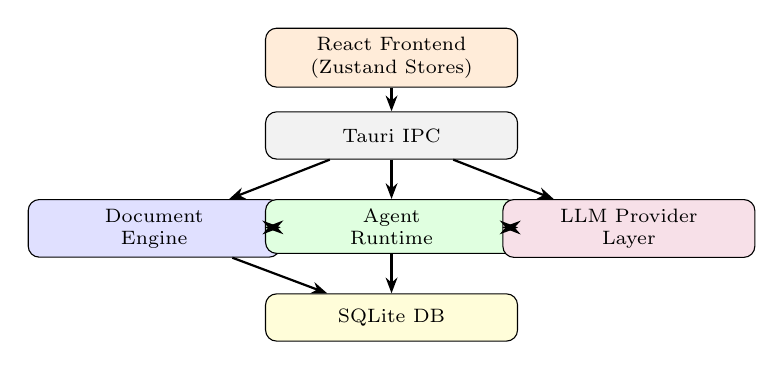
\begin{tikzpicture}[
    node distance=0.3cm,
    box/.style={draw, rounded corners, minimum width=3.2cm, minimum height=0.6cm, align=center, font=\scriptsize},
    layer/.style={draw, dashed, rounded corners, inner sep=0.2cm},
    arr/.style={-{Stealth[length=2mm]}, thick},
    >=Stealth
]
% Frontend
\node[box, fill=orange!15] (fe) {React Frontend\\(Zustand Stores)};

% IPC
\node[box, fill=gray!10, below=of fe] (ipc) {Tauri IPC};

% Backend boxes
\node[box, fill=blue!12, below left=0.5cm and -0.2cm of ipc] (doc) {Document\\Engine};
\node[box, fill=green!12, below=0.5cm of ipc] (agent) {Agent\\Runtime};
\node[box, fill=purple!12, below right=0.5cm and -0.2cm of ipc] (llm) {LLM Provider\\Layer};

% DB
\node[box, fill=yellow!15, below=0.5cm of agent] (db) {SQLite DB};

% Arrows
\draw[arr] (fe) -- (ipc);
\draw[arr] (ipc) -- (doc);
\draw[arr] (ipc) -- (agent);
\draw[arr] (ipc) -- (llm);
\draw[arr] (agent) -- (db);
\draw[arr] (doc) -- (db);
\draw[arr, <->] (agent) -- (llm);
\draw[arr, <->] (agent) -- (doc);

\end{tikzpicture}
\caption{TGG system architecture. The React frontend communicates with the Rust backend via Tauri IPC. The backend comprises three core subsystems: the Document Engine (parsing), the Agent Runtime (exploration), and the LLM Provider Layer (multi-provider abstraction). All persistent state resides in a local SQLite database.}
\label{fig:architecture}
\end{figure}

\subsection{Universal Document Tree}

The Universal Document Tree (UDT) is the central data structure of TGG. Every ingested document, regardless of its original format, is parsed into a tree of typed nodes:

\begin{equation}
\text{Node} = \langle id, \tau, c, M, \mathbf{ch}, \mathbf{R}, s \rangle
\label{eq:node}
\end{equation}

\noindent where $id$ is a unique identifier, $\tau \in \mathcal{T}$ is the node type drawn from the type vocabulary $\mathcal{T} = \{\texttt{Root}, \texttt{Section}, \texttt{Heading}, \texttt{Paragraph}, \texttt{Table}, \texttt{TableRow}, \texttt{TableCell}, \texttt{Image}, \texttt{CodeBlock}, \texttt{ListItem}, \texttt{Link}\}$, $c$ is the full text content, $M$ is a metadata dictionary (e.g., heading level, page number, programming language), $\mathbf{ch}$ is an ordered list of child node identifiers, $\mathbf{R}$ is a set of typed relations to other nodes, and $s$ is an optional summary.

A document tree $T = \langle D, r, \mathcal{N} \rangle$ consists of document metadata $D$ (name, type, timestamps), a root node identifier $r$, and a node map $\mathcal{N}: id \rightarrow \text{Node}$.

Relations $\mathbf{R}$ are typed edges: $R = \langle \text{target\_id}, \rho, \ell \rangle$ where $\rho \in \{\texttt{References}, \texttt{DependsOn}, \texttt{SimilarTo}, \texttt{Contains}, \texttt{LinkedTo}\}$ and $\ell$ is an optional label. These enable cross-document and cross-section navigation.

\textbf{Parser Architecture.} TGG implements six format-specific parsers, each producing UDT output:

\begin{itemize}
    \item \textbf{PDF}: Page-aware extraction with heuristic heading detection. Headings are identified via three rules: keyword prefixes (``Chapter'', ``Section''), ALL-CAPS short lines ($\leq 80$ characters), and short capitalized lines not ending in punctuation ($\leq 60$ characters). A section stack maintains proper nesting.
    \item \textbf{Markdown}: Event-driven parsing via pulldown-cmark, tracking heading hierarchy with a section stack that pops when a heading of equal or higher level is encountered.
    \item \textbf{Word (DOCX)}: XML extraction from the ZIP container, with paragraph style-based heading detection and recursive table structure preservation.
    \item \textbf{Spreadsheet (XLSX/XLS/ODS)}: Sheet-level decomposition into Table $\rightarrow$ TableRow $\rightarrow$ TableCell hierarchies, with type-aware cell value conversion.
    \item \textbf{Source Code}: Language-tagged 60-line code blocks with line range metadata, supporting 20+ programming languages.
    \item \textbf{Plain Text}: Double-newline paragraph splitting with word count metadata.
\end{itemize}

The section stack algorithm (Algorithm~\ref{alg:sectionstack}) ensures that all parsers produce properly nested trees, regardless of input format idiosyncrasies.

\begin{algorithm}[t]
\caption{Section Stack Nesting Algorithm}
\label{alg:sectionstack}
\begin{algorithmic}[1]
\REQUIRE Document elements $E$, root node $r$
\STATE $\text{stack} \leftarrow [(0, r.\text{id})]$
\FOR{each element $e \in E$}
    \IF{$e$ is a heading at level $\ell$}
        \WHILE{$\text{stack.top().level} \geq \ell$}
            \STATE $\text{stack.pop()}$
        \ENDWHILE
        \STATE $\text{parent} \leftarrow \text{stack.top().id}$
        \STATE $n \leftarrow \text{Node}(\texttt{Section}, e.\text{text}, \{\text{level}: \ell\})$
        \STATE Add $n$ as child of $\text{parent}$
        \STATE $\text{stack.push}((\ell, n.\text{id}))$
    \ELSE
        \STATE $\text{parent} \leftarrow \text{stack.top().id}$
        \STATE $n \leftarrow \text{Node}(e.\text{type}, e.\text{content}, e.\text{metadata})$
        \STATE Add $n$ as child of $\text{parent}$
    \ENDIF
\ENDFOR
\end{algorithmic}
\end{algorithm}

\subsection{Agent Exploration Protocol}

The core of TGG is the agent exploration loop, where an LLM equipped with navigation tools iteratively explores the document tree to gather evidence for answering a user query. The protocol is formalized in Algorithm~\ref{alg:agentloop}.

\begin{algorithm}[t]
\caption{Agent Exploration Loop}
\label{alg:agentloop}
\begin{algorithmic}[1]
\REQUIRE Query $q$, document tree $T$, LLM provider $\mathcal{L}$
\STATE $P \leftarrow \text{PreprocessQuery}(q)$ \COMMENT{Intent, terms, budget}
\STATE $\text{ctx} \leftarrow \text{ExplorationContext}()$
\STATE $\text{msgs} \leftarrow [\text{SystemPrompt}(T), \text{UserQuery}(q)]$
\STATE $\text{nudges} \leftarrow 0$
\IF{$P.\text{intent}$ requires pre-search}
    \STATE Execute \textsc{SearchContent} for each search term
\ENDIF
\FOR{$\text{step} = 1$ to $P.\text{max\_steps}$}
    \IF{CancelFlag is set}
        \RETURN \textit{cancelled}
    \ENDIF
    \STATE $\text{resp} \leftarrow \mathcal{L}.\text{chat}(\text{msgs}, \text{tools})$
    \STATE Update token/latency accounting
    \IF{$\text{resp}$ contains no tool calls}
        \IF{$\text{ctx.step\_count} < P.\text{min\_tools}$ \AND $\text{nudges} < 2$}
            \STATE Append nudge message; $\text{nudges}$++
            \STATE \textbf{continue}
        \ELSE
            \STATE \textbf{break} \COMMENT{Agent ready to answer}
        \ENDIF
    \ENDIF
    \FOR{each tool call $t$ in $\text{resp}$}
        \STATE $\text{result} \leftarrow \text{ExecuteTool}(t, T)$
        \STATE $\text{ctx.record}(t.\text{node\_ids}, \text{result})$
        \STATE Emit exploration step event
        \STATE Append tool result to msgs
    \ENDFOR
    \STATE Cap msgs to 60 messages
\ENDFOR
\STATE $\text{answer} \leftarrow \mathcal{L}.\text{synthesize}(\text{msgs})$
\STATE $\text{ctx.compute\_relevance\_scores}()$
\RETURN $\text{answer}$, $\text{ctx}$
\end{algorithmic}
\end{algorithm}

\textbf{Navigation Tools.} The agent is equipped with seven tools, each designed for a specific tree navigation operation:

\begin{enumerate}
    \item \textsc{TreeOverview}$(T)$: Returns the immediate children of the root node with content previews ($\leq 100$ characters), providing a structural overview analogous to a table of contents.
    \item \textsc{ExpandNode}$(n)$: Returns the full content of node $n$ and all its direct children, enabling one-level-at-a-time depth exploration.
    \item \textsc{SearchContent}$(q, \text{scope}?)$: Case-insensitive substring search across the tree, optionally scoped to a subtree rooted at a specified node. Returns matching node summaries.
    \item \textsc{GetRelations}$(n)$: Returns all typed relations from node $n$, enabling cross-reference following.
    \item \textsc{GetImage}$(n)$: Retrieves image node metadata and file path for vision-capable LLMs.
    \item \textsc{CompareNodes}$(a, b)$: Returns full content of two nodes side-by-side, enabling cross-document or cross-section comparison.
    \item \textsc{GetNodeContext}$(n)$: Returns the path from root to node $n$ (breadcrumb chain), providing hierarchical positioning context.
\end{enumerate}

\textbf{Scoped Search.} The \textsc{SearchContent} tool supports subtree scoping via a descendant check: given a scope node $s$, only nodes $n$ where $n$ is a descendant of $s$ are searched. This is implemented as a BFS traversal from $s$ with a visited set for cycle protection. Subtree scoping enables the agent to narrow its search after identifying a relevant section via \textsc{TreeOverview}, mimicking the human pattern of first navigating to a section and then searching within it.

\subsection{Query-Adaptive Budget Estimation}

Not all queries require the same exploration depth. A simple factual lookup may need two tool calls, while a comprehensive comparison across document sections may require fifteen. TGG addresses this with a query preprocessor that classifies intent and estimates exploration complexity.

The preprocessor classifies each query into one of six intent categories based on keyword matching: \texttt{Summarize}, \texttt{Entity}, \texttt{Factual}, \texttt{Comparison}, \texttt{ListExtract}, or \texttt{Specific}. It then computes a complexity score:

\begin{equation}
\text{complexity} = b_\tau + \alpha_w + \alpha_t
\end{equation}

\noindent where $b_\tau$ is the base cost for intent type $\tau$ (ranging from 2 for entity lookups to 4 for comparisons), $\alpha_w$ is a word count boost (+1 for $>$10 words, +2 for $>$20 words), and $\alpha_t$ is a term diversity boost (+1 for $>$2 unique search terms, +2 for $>$4). The recommended maximum steps are computed as:

\begin{equation}
\text{max\_steps} = \text{clamp}(\text{complexity} \times 2 + 4, \; 6, \; 15)
\end{equation}

This adaptive budgeting prevents token waste on simple queries while allowing thorough exploration for complex ones. The minimum tool call threshold ($P.\text{min\_tools}$, set to 2--4 based on intent) ensures the agent does not short-circuit exploration prematurely.

\subsection{Multi-Provider LLM Abstraction}

TGG abstracts LLM communication behind a provider trait with a unified interface for chat completion with tool calling. The system supports ten providers: Groq, Google Gemini, OpenRouter, AgentRouter, Anthropic, OpenAI, DeepSeek, xAI/Grok, Qwen, and Ollama (local).

A critical implementation challenge is \textit{message format divergence}. Different providers represent tool calls and tool results in incompatible formats:

\begin{itemize}
    \item OpenAI-compatible providers (Groq, OpenRouter, DeepSeek, xAI, Qwen, Ollama) use \texttt{tool\_calls} arrays in assistant messages and \texttt{role: "tool"} for results.
    \item Anthropic uses \texttt{tool\_use} content blocks and wraps tool results in user messages with \texttt{tool\_result} blocks.
    \item Google Gemini uses \texttt{functionCall} parts and requires tool results as JSON objects within \texttt{functionResponse} parts, with consecutive tool messages merged.
\end{itemize}

TGG implements a normalization layer that converts between an internal message representation and each provider's native format, enabling seamless provider switching without changes to the agent logic.

\subsection{Exploration Context and Relevance Scoring}

The agent maintains an \texttt{ExplorationContext} that tracks visited nodes, per-node visit counts, output summaries, and cumulative token/cost metrics. After exploration completes, TGG computes a relevance score for each visited node:

\begin{equation}
\text{relevance}(n) = 0.6 \cdot \frac{\text{visits}(n)}{\max_{n'} \text{visits}(n')} + 0.4 \cdot \min\!\left(\frac{|\text{summary}(n)|}{200}, 1\right)
\label{eq:relevance}
\end{equation}

This score combines visit frequency (indicating the agent's repeated interest) with output richness (indicating substantive content extraction). Relevance scores enable post-hoc visualization of the exploration path and support future query routing by identifying which document regions were most informative.

\subsection{Local Tracing and Evaluation}

TGG implements a local tracing framework inspired by Langfuse, storing per-query traces with step-level granularity. Each trace records: the provider used, total and per-step token counts (input and output separately), cost computed from a pricing table, latency per LLM turn (distributed across tool calls within that turn), and the sequence of tools invoked with their inputs and outputs. An evaluation layer supports metric-based scoring (0--1 scale) per trace, adopting metrics analogous to those in RAGAS~\cite{es2024ragas} (faithfulness, answer relevance, context precision) but computed locally without cloud dependency. This enables longitudinal quality analysis while preserving full data sovereignty.

% =====================================================================
% V. IMPLEMENTATION
% =====================================================================
\section{Implementation}

TGG is implemented as a desktop application using Tauri v2 (Rust backend with WebView frontend). The Rust backend uses the Tokio async runtime for concurrent LLM API communication and document processing. The frontend is built with React 19 and TypeScript, using Zustand for state management across four domain stores (chat, documents, settings, traces).

\subsection{Database Design}

All persistent state is stored in a SQLite database with WAL (Write-Ahead Logging) mode for concurrent read-write safety. The schema comprises eight tables: \texttt{documents} (storing the full serialized UDT as JSON), \texttt{conversations}, \texttt{messages}, \texttt{traces}, \texttt{exploration\_steps}, \texttt{evals}, \texttt{settings}, \texttt{providers}, and \texttt{bookmarks}. Document trees are serialized as JSON within the \texttt{tree\_json} column, enabling schema-free evolution of the node structure without database migrations. Queries by document ID are indexed for sub-millisecond lookup.

\subsection{Cancel-Safe Async Exploration}

Tauri's IPC mechanism does not support native invocation cancellation. TGG addresses this with a shared \texttt{Arc<AtomicBool>} cancel flag managed as Tauri application state. The frontend sets this flag via an \texttt{abort\_query} command; the agent loop checks the flag at the top of each iteration using \texttt{SeqCst} ordering (sequential consistency), ensuring all threads observe the cancellation immediately. This design enables instant query cancellation without partial state corruption or exception unwinding.

\subsection{Streaming Response Emission}

LLM responses are streamed to the frontend via Tauri's event system. The backend emits structured events at three granularities: \texttt{exploration-step-start} and \texttt{exploration-step-complete} events during tool execution (enabling real-time visualization of the agent's exploration path), and \texttt{chat-token} events for word-level response streaming. Tokens are emitted in chunks of three words with explicit yields between chunks, preventing UI thread blocking while maintaining natural reading rhythm.

\subsection{Tree Visualization}

The frontend implements an SVG-based tree visualization using the Reingold-Tilford layout algorithm. Nodes are positioned with 70px horizontal spacing and 80px vertical spacing per depth level, with the display capped at three levels to prevent visual overload. Nodes are color-coded by type (sections in blue, paragraphs in purple, tables in green, code blocks in pink) and dynamically highlighted as the agent visits them during exploration, providing a real-time visual trace of the agent's navigation path.

\subsection{Codebase Metrics}

The core implementation comprises approximately 5,000 lines of Rust (parsers: 679 lines, agent runtime: 347 lines, tools: 240 lines, LLM providers: 1,500+ lines across ten implementations, commands/IPC: 1,001 lines, database: 400+ lines) and 3,000+ lines of TypeScript/React for the frontend. All dependencies are open-source.

% =====================================================================
% VI. COMPARATIVE ANALYSIS
% =====================================================================
\section{Comparative Analysis}

We present a systematic comparative analysis of TGG against three baseline approaches: Traditional RAG (embedding-based retrieval), Agentic RAG (agent-controlled retrieval over vector stores), and Graph RAG (entity graph-based retrieval). We evaluate across twelve dimensions organized into four categories: structural preservation, retrieval quality, operational characteristics, and practical constraints. Table~\ref{tab:comparison} summarizes the analysis.

\begin{table*}[t]
\centering
\caption{Comparative Analysis Across Twelve Dimensions}
\label{tab:comparison}
\footnotesize
\begin{tabular}{@{}p{2.8cm}p{3.2cm}p{3.2cm}p{3.2cm}p{3.2cm}@{}}
\toprule
\textbf{Dimension} & \textbf{Traditional RAG} & \textbf{Agentic RAG} & \textbf{Graph RAG} & \textbf{TGG (Ours)} \\
\midrule
\multicolumn{5}{l}{\textit{Structural Preservation}} \\
\midrule
Hierarchy retention & None (flat chunks) & None (flat chunks) & Partial (entity clusters) & Full (native tree) \\
Cross-reference support & None & None & Entity-level only & Typed relations \\
Table structure & Destroyed & Destroyed & Not applicable & Preserved (row/cell) \\
\midrule
\multicolumn{5}{l}{\textit{Retrieval Quality}} \\
\midrule
Multi-hop reasoning & Limited to $k$ chunks & Agent-driven, iterative & Community summaries & Tree traversal \\
Scoped search & Global only & Global with reranking & Subgraph filtering & Subtree scoping \\
Context coherence & Chunk-level & Chunk-level & Summary-level & Section-level \\
\midrule
\multicolumn{5}{l}{\textit{Operational Characteristics}} \\
\midrule
Indexing cost & Embedding model + vector DB & Embedding model + vector DB & LLM entity extraction & Deterministic parsing only \\
Query-time LLM calls & 1 (generation only) & 2--5 (retrieval + generation) & 1--2 & 3--15 (exploration + synthesis) \\
Infrastructure & Vector DB required & Vector DB required & Graph DB + vector DB & SQLite only \\
\midrule
\multicolumn{5}{l}{\textit{Practical Constraints}} \\
\midrule
Latency & Low (single retrieval) & Medium (iterative) & Medium & Higher (multi-turn) \\
Privacy & Depends on hosting & Depends on hosting & Depends on hosting & Fully local \\
Provider flexibility & Tied to embedding model & Tied to embedding model & Tied to extraction model & Any LLM provider \\
\bottomrule
\end{tabular}
\end{table*}

\subsection{Structural Preservation Analysis}

The most significant advantage of TGG is the preservation of document hierarchy throughout the retrieval process. To illustrate concretely, consider how each approach handles a 50-page technical specification with nested sections, cross-referenced tables, and an appendix.

\textbf{Traditional RAG} splits this document into approximately 100--200 chunks, destroying all section nesting. A table spanning two pages becomes two disconnected chunks; neither contains the table header with column definitions. A section that references ``see Appendix B.3'' provides no mechanism for the retriever to follow this reference.

\textbf{Graph RAG} extracts entities (component names, parameters, standards) and their relations, creating a knowledge graph. This preserves entity-level relationships but not the document's own organizational structure. The graph encodes that ``Component X relates to Thermal Constraint Y'' but not that this information appears in Section 4.2, subsection ``Operating Parameters,'' which the engineer may need for citation or verification purposes.

\textbf{TGG} parses the specification into a tree that mirrors its actual structure: Root $\rightarrow$ Chapters $\rightarrow$ Sections $\rightarrow$ Subsections, with Table and Image nodes as children of their containing sections. The agent can navigate this tree exactly as a human reader would: overview the structure, locate the relevant chapter, expand into the specific section, and follow cross-references via typed relations.

\subsection{Retrieval Quality Analysis}

We analyze retrieval quality through three lenses: multi-hop reasoning, context coherence, and failure mode analysis.

\textbf{Multi-hop Reasoning.} Questions requiring information from multiple document locations are a known weakness of single-shot retrieval~\cite{liu2024lostmiddle}. Traditional RAG retrieves the top-$k$ chunks independently, providing no mechanism for following logical chains. TGG's agent can perform multi-hop reasoning explicitly: \textsc{TreeOverview} $\rightarrow$ \textsc{ExpandNode} on Section~4 $\rightarrow$ \textsc{SearchContent} for ``thermal'' within that subtree $\rightarrow$ \textsc{GetRelations} to find the referenced appendix table $\rightarrow$ \textsc{ExpandNode} on the appendix. Each step is recorded in the trace, providing a verifiable chain of evidence.

\textbf{Context Coherence.} When traditional RAG retrieves chunks, each chunk carries no information about its position within the document. A paragraph about exceptions may be retrieved without the rule it modifies. TGG maintains section-level context through the tree structure: when the agent expands a node, it receives both the node content and its children, preserving the parent-child semantic relationship. The \textsc{GetNodeContext} tool provides the full path from root to any node, enabling the agent to understand exactly where a piece of information sits within the document hierarchy.

\textbf{Failure Mode Analysis.} Traditional RAG's primary failure mode is \textit{semantic mismatch}: the query embedding fails to align with the relevant chunk embedding, even when the content is objectively relevant. This manifests as both false negatives (relevant chunks not retrieved) and false positives (irrelevant chunks retrieved). TGG replaces this with a different failure mode: \textit{exploration incompleteness}, where the agent fails to navigate to the relevant node within its step budget. This failure mode is more predictable (it correlates with query complexity and document size) and more addressable (by increasing the step budget or providing more specific search terms).

\subsection{Operational Analysis}

\textbf{Indexing Cost.} Traditional and Agentic RAG require running every document through an embedding model and storing the resulting vectors in a specialized database. Graph RAG additionally requires LLM-based entity extraction, which can cost \$2--5 per 1M tokens. TGG's indexing is purely deterministic parsing---no LLM calls, no embeddings, no specialized databases. A 100-page PDF is parsed in approximately 200ms on commodity hardware. This eliminates embedding drift, removes the need to re-embed when switching models, and reduces indexing from minutes to milliseconds.

\textbf{Query-Time Cost.} TGG's trade-off is increased query-time LLM usage. Where traditional RAG makes a single LLM call (the generation step), TGG makes 3--15 calls (exploration turns plus final synthesis). At current API pricing, a typical TGG query with 6 exploration steps using a cost-efficient model (e.g., Groq with Llama-3.3-70B) costs approximately \$0.001--0.005, compared to \$0.0005--0.002 for a single RAG generation call. This 2--5x cost increase is offset by zero indexing cost and zero vector database maintenance.

\textbf{Privacy.} TGG's local-first architecture stores all data in a local SQLite database. No document content is transmitted to external services except during LLM API calls for exploration, and users can choose fully local providers (Ollama) for complete data sovereignty. The tracing framework operates entirely locally, with no cloud telemetry dependency.

\subsection{Limitations Comparison}

Table~\ref{tab:limitations} presents an honest comparison of limitations across approaches.

\begin{table}[t]
\centering
\caption{Limitations Comparison}
\label{tab:limitations}
\footnotesize
\begin{tabular}{@{}p{2.0cm}p{5.8cm}@{}}
\toprule
\textbf{Approach} & \textbf{Key Limitations} \\
\midrule
Traditional RAG & Structural erasure, chunk boundaries, embedding drift, vector DB maintenance \\
\addlinespace
Agentic RAG & Inherits embedding limitations, agent reliability, compounding errors \\
\addlinespace
Graph RAG & Expensive indexing (LLM entity extraction), entity-centric bias, poor for non-entity queries \\
\addlinespace
TGG (Ours) & Higher query latency, no semantic similarity for fuzzy matching, limited by parser heuristics, step budget caps large documents \\
\bottomrule
\end{tabular}
\end{table}

TGG's most significant limitation is the absence of semantic similarity. If a user asks about ``environmental impact'' and the document discusses ``ecological footprint'' without using the query terms, TGG's keyword-based \textsc{SearchContent} tool will not find it. Traditional RAG's embeddings would capture this semantic equivalence. This limitation suggests that a hybrid approach---tree-grounded exploration augmented with optional semantic search at leaf nodes---may be the optimal configuration for production systems, a direction we leave for future work.

% =====================================================================
% VII. DISCUSSION
% =====================================================================
\section{Discussion}

\subsection{When to Use TGG}

TGG is best suited for scenarios where document structure carries significant informational value: technical specifications, legal contracts, academic papers, codebases, and regulatory filings. In these domains, the hierarchical organization of content is not incidental but \textit{constitutive}---the structure itself conveys meaning (e.g., a clause's legal force depends on its position within a contract's section hierarchy). For corpora consisting primarily of unstructured prose (e.g., social media posts, chat logs), traditional RAG's flat retrieval is likely sufficient and more cost-efficient.

\subsection{Scalability Considerations}

TGG's current implementation stores entire document trees as serialized JSON in SQLite. For corpora of thousands of documents, the agent must first identify the relevant document before exploring its tree. This two-stage process (document selection $\rightarrow$ tree exploration) is currently manual (the user selects documents). Scaling to large corpora would require a lightweight document-level index---potentially using embeddings at the document level while retaining tree-based exploration at the document level, combining the strengths of both paradigms.

\subsection{Parser Robustness}

The PDF parser relies on heuristic heading detection rather than machine learning-based document layout analysis. While effective for well-structured documents, this approach may misclassify headings in documents with unconventional formatting. The system's modular parser architecture allows individual parsers to be upgraded independently; a future direction is integrating ML-based layout analysis (e.g., LayoutLM) for more robust PDF parsing while maintaining the same UDT output schema.

\subsection{Threats to Validity}

Our comparative analysis is analytical rather than empirical. We do not report benchmark scores on standardized datasets, as TGG's evaluation requires structure-aware benchmarks that do not yet exist---current RAG benchmarks such as CRAG~\cite{yang2024crag}, RAGBench~\cite{friel2024ragbench}, and MIRAGE~\cite{park2025mirage} evaluate over flat document collections and do not measure structural preservation or hierarchical retrieval quality. Developing such benchmarks is an important direction for future work. Additionally, the quality of TGG's retrieval depends on the LLM agent's tool-use capabilities, which vary significantly across providers and models.

% =====================================================================
% VIII. CONCLUSION AND FUTURE WORK
% =====================================================================
\section{Conclusion and Future Work}

We have presented Tree-Grounded Generation (TGG), a retrieval paradigm that replaces embedding-based similarity search with agentic exploration of structured document trees. TGG addresses three fundamental limitations of traditional RAG---chunk boundary artifacts, embedding fragility, and structural erasure---by preserving document hierarchy in a Universal Document Tree and equipping an LLM agent with seven specialized navigation tools to explore it deliberately.

Our comparative analysis across twelve dimensions demonstrates that TGG offers superior structural preservation, enables verifiable multi-hop reasoning through explicit tree traversal, and eliminates the operational overhead of vector database maintenance. These advantages come at the cost of increased query-time latency and the absence of semantic similarity for fuzzy matching.

We identify several directions for future work:

\begin{itemize}
    \item \textbf{Hybrid retrieval}: Combining tree-grounded exploration with optional semantic search at leaf nodes to address the fuzzy matching limitation.
    \item \textbf{Relation inference}: Using LLMs to automatically populate cross-reference relations between nodes during indexing.
    \item \textbf{Structure-aware benchmarks}: Developing evaluation datasets that explicitly measure hierarchical retrieval quality, analogous to CRAG for flat retrieval.
    \item \textbf{Multi-document exploration}: Extending the agent protocol with cross-tree navigation tools for corpora-level exploration.
    \item \textbf{Adaptive parser selection}: ML-based document layout analysis (e.g., LayoutLM) for robust PDF parsing while maintaining the UDT output schema.
\end{itemize}

TGG demonstrates that embedding-based similarity is not the only viable retrieval mechanism for grounding LLM outputs. As documents grow in structural complexity and domain specificity, we anticipate increasing demand for retrieval systems that respect and exploit document structure rather than erasing it.

% =====================================================================
% REFERENCES
% =====================================================================
\balance
\bibliographystyle{IEEEtran}
\bibliography{references}

\end{document}
